\documentclass[a4paper, 12pt]{article}

\usepackage{fancyhdr}
\pagestyle{fancy}
\lhead{PROJET : Forteresse}
\lfoot{Info Sup}
\rfoot{EPITA 2016}
\renewcommand{\footrulewidth}{0.3mm}

\usepackage[french]{babel}
\usepackage{listings}
\usepackage[T1]{fontenc}
\usepackage{eurosym}
\usepackage{setspace}
\usepackage{caption}
\usepackage{titlesec}

\usepackage[utf8]{inputenc}
\usepackage{graphicx}

\setcounter{secnumdepth}{4}

\titleformat{\paragraph}
{\normalfont\normalsize\bfseries}{\theparagraph}{1em}{}
\titlespacing*{\paragraph}
{0pt}{3.25ex plus 1ex minus .2ex}{1.5ex plus .2ex}

\renewcommand{\baselinestretch}{1.5}
\begin{document}
\begin{titlepage}
  \begin{sffamily}
  \begin{center}

    % Upper part of the page. The '~' is needed because \\
    % only works if a paragraph has started.

    \textsc{\Huge Rapport soutenance 2}\\[3cm]

    \textsc{\LARGE Projet:}\\[1.5cm]

    % Title
	\centerline{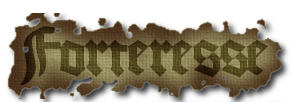
\includegraphics{coollogo_com-19602433.png}}
	\vfill{
	\centerline{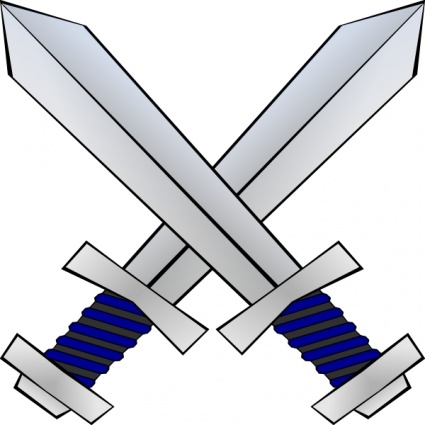
\includegraphics[scale=0.4]{crossed-swords-clip-art-48219.jpg}}}

    % Author and supervisor
    \begin{minipage}{0.4\textwidth}
      \begin{flushleft} \large	
      
      \end{flushleft}
    \end{minipage}
	\begin{flushleft}\vfill
      {
       \textsc{Chatelus} Florian - \emph{chatel\_f} \\
       \textsc{Henric} Arnaud - \emph{henric\_a}\\
       \textsc{Sarkar} Riday - \emph{sarkar\_r}\\
       }
    \end{flushleft}	
  \end{center}
  \end{sffamily}
\end{titlepage}

\begin{spacing}{1.0}
	\tableofcontents
\end{spacing}

\newpage
\section{Introduction}
Dans le cadre de de notre première année à EPITA, nous devons réaliser un projet informatique de fin d’année qui doit montrer l’application de nos connaissances dans le domaine de la programmation. Pour réaliser ce projet, nous avions formé un groupe composé de quatre étudiants. Actuellement, notre groupe n’est composé que de trois étudiants puisqu’un membre du groupe à quitté l’école.  
Le sujet étant libre, nous avons décidé de réaliser un jeu vidéo nommé Forteresse. C’est un jeu du type Tower Defense. La présentation du jeu est détaillée dans la reprise du cahier des charges.  
	\par Le présent document est  le rapport de projet  qui retrace les différents cheminements de création de ce projet  et il présente surtout le jeu.  Nous avons donc décrit les différentes tâches réalisées ainsi que les problèmes rencontrés et les solutions trouvées pour résoudre ces problèmes.
	\par Le plan de notre rapport sera divisé en trois parties. La première étant consacrée à la reprise du cahier des charges, la deuxième est consacrée à la présentation du jeu et la troisième, quant à elle, est consacrée au bilan personnel de chaque étudiant faisant partie de ce groupe.


\newpage
\section{Cahier des charges}
\subsection{Les origines du projet}
Nous avons choisi de réaliser un jeu plutôt qu’un logiciel car nous avons deux membres dans le groupe qui ont déjà réalisé un jeu en Terminale dans le cadre d’un projet en groupe. Même si le projet achevé en ISN par ces deux derniers n’est pas comparable avec ce qui nous attend ce semestre en INFO SUP, ce sera toujours une aide non-négligeable.
\par Une fois que la nature du projet était choisi, nous avons réfléchi longuement sur le type de jeu que nous allons réaliser. Notre expérience en tant que joueur nous donnait un large choix parmi les types de jeu possibles comme un RPG (Role Playing Game), RTS (Real Time Strategy) ou encore un Tower Defense . 

		\subsubsection{Présentation}
		\par Notre jeu sera basé sur le principe du \textit{tower defense}. Qu'est-ce que 			cela signifie? Un \textit{tower defense}, est un jeu qui comme son nom l'indique 			aura comme objectif de défendre un point donné. Le but du jeu sera donc de défendre 		un cristal qui alimente la porte de l'endroit que nous souhaitons protéger.  
		\subsubsection{Déroulement d'une partie}
		Une partie se déroulera en deux phases qui se répéteront, a chaque vague d'ennemis.\\
		\centerline{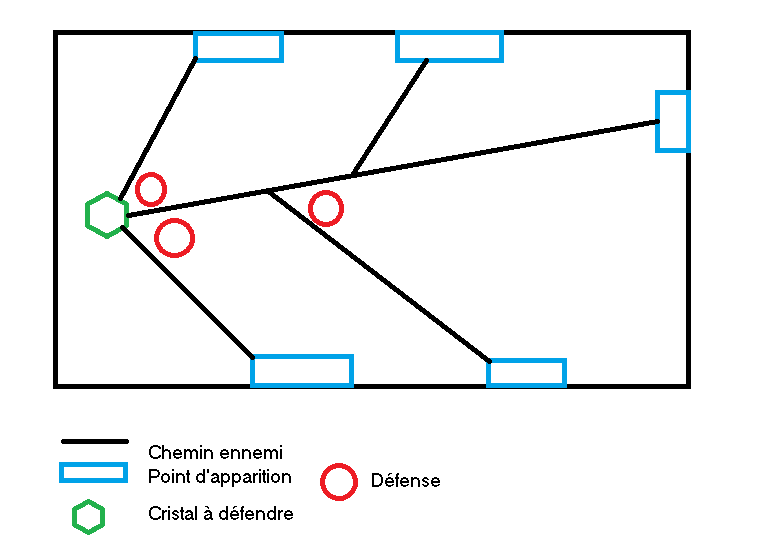
\includegraphics[scale=0.55]{Plan.png}}
		\par La première est la phase que nous appellerons \textit{phase de préparation}, elle consiste à préparer ses défenses, en les positionnant de façon stratégique, les améliorant ou en les réparant. Cette phase sera d'une importance capital pour assurer une victoire lors de la phase suivante. Une fois que vous serez fin prêt pour le combat, il vous suffira d'appuyer sur prêt et la deuxième phase commencera une fois tout les joueurs prêt.
		\par Nous arrivons donc en deuxième phase, la \textit{phase de combat}, qui va déclencher l'action. Des créatures vont apparaitre à des points précis de la carte et vont converger vers le ou les cristaux. Le joueur pourra donc durant cette phase attaquer les monstres et tenter de les détruire et/ou continuer à poser, améliorer et réparer ses constructions mais avec des malus d'incantation.
		\par Tous les certains nombre de cycle, au terme de ces deux phases, un monstre plus imposant apparaitra, et le joueur devra s'en défaire afin de remporter la manque et d'obtenir des objets.
		\subsubsection{Multijoueur}
		Le mode multijoueur consistera en un mode CO-OP. Vous devrez \^etre capable de jouer en \'equipe afin d'affronter vos adversaires. Pour cela, vous commencerez la partie c\^ote \'a c\^ote. Vous ne pouvez combattre seulement des IA. Le mode multijoueur consiste en un mode en \'equipe et non pas en 1vs1 contre un ami.
		\par Chaque joueur pourra int\'eragir avec l'environnement. Leurs constructions et leurs objectifs sont communs tandis que toutes leurs caract\'eristiques telles que leur monnaie et leur vie sont s\'epar\'ees.
		\subsubsection{L'interface}
		L’interface permettra au joueur d'être renseignée à tout moment sur : 
		\begin{itemize}
		\item Le temps écoulé.
		\item Sa jauge de vie.
		\item L’arme dont il est en possession , ainsi que les  munitions dont il dispose.
		\item L’argent qu’il possède pour acheter de nouvelles tours ou armes.
		\end{itemize}
		\subsubsection{L'arsenal de défense}
		Nous utiliserons donc différents types d’armes de type médiéval fantastique.
Les armes seront donc accessible en la ramassant sur un bosse ou bien  suite à un achat du joueur, elles pourront être améliorer, durant la partie. On distinguera plusieurs types d’armes tel que:
	\begin{itemize}
	\item Les épées.
	\item Les arcs.
	\item Les bâtons.
	\end{itemize}
Les défenses fixes seront achetable grâce a l’argent gagné durant la partie. Les défenses seront comme les armes améliorables. Ces dernières seront autonomes et feront partie de l’IA. On pourra y trouver:
	\begin{itemize}
	\item Des tourelles.
	\item Des pièges.
	\item Des auras.
	\end{itemize}
\newpage
\subsection{Découpage du projet}
	\subsubsection{Le graphisme}
		\subsubsection{La 3D}
		Étant donné sa gratuité, nous allons utiliser Blender pour réaliser des modèles 3D. Ce logiciel va nous permettre de modéliser les différents personnages de notre jeu et de faire les diverses textures de l’environnement du jeu.

		\subsubsection{La 2D}
		La 2D de notre jeu sera principalement représenté par l'interface graphique du joueur. En effet, le joueur aura besoin d'avoir des informations et de repère visuel afin d'interagir correctement avec son environnement et d'avoir une expérience de jeu la meilleure possible. La 2D pourra également jouer un rôle important dans les menus
	\subsubsection{Audio}
	L’audio gère évidemment tous les sons. De bruitages dans le jeu à musique dans les menus, nous devrons trouver des sons qui s’adaptent au contexte médiéval.

	\subsubsection{Le réseau}
	Le réseau consistera tout simplement a implémenter un mode multijoueur, afin que les joueurs puisse jouer ensemble en ligne ou bien en réseau local.
	\subsubsection{L'intelligence artificiel}
	Pour définir l’IA, nous allons créer différents niveaux de difficultés. Le but est que l’IA détruise le cristal que nous devons protéger, ainsi, l’IA est l’ennemie. Il contrôle plusieurs personnages. Nous devons coder un IA capable de se déplacer vers le cristal, mais également de combattre contre l’utilisateur, de mourir tué par le héros ou les tourelles. 

	\subsubsection{Le menu}
	Nous tenterons de créer un menu accessible et design. Il devra permettre d'accéder au lancement d’une nouvelle partie, aux options, ainsi qu’au mode multi-joueur. 
	\subsubsection{Le site}
	Modéliser un site web avec une présentation générale des créateurs et de la création (chronologie, problèmes, solutions…). Ajouter des images du jeu. Expliquer les règles.  Donner les références utiles pour notre réalisation. Permettre le téléchargement du jeu aux utilisateurs, et mettre à disposition le rapport ainsi que le jeu en version lite.
	\subsubsection{Gameplay}
	Le gameplay consiste à coder tous les mouvements de notre héros, soit le personnage que l’on contrôle… Il devra être capable de donner des coups, construire des tours, courir, sauter, et bien sûr, se déplacer à n’importe qu’elle point accessible de la map. Le gameplay consiste également à coder la caméra suivant notre héros. Ce jeu se jouant à la troisième personne, la caméra devra être capable de toujours regarder le héros de derrière et de le suivre dans tous ses mouvements. On devra ici géré également tous les problèmes de collision.
	\subsubsection{Animation}
	L’animation est le moyen de rendre les mouvements des personnages fluides et réalistes. Chaque mouvement devra être animé, les jambes lorsqu’un personnage se déplace, les bras lorsqu’il combat, etc...

\newpage

\subsection{Répartition des tâches}
Nous avons décidé d’attribuer chaque tâche à au moins deux personnes car ainsi chaque membre réalise plusieurs tâches et peut apprendre des choses de domaines différents . De plus, si un membre rencontre des difficultés et se retrouve bloqué pour réaliser une tâche, son coéquipier peut venir en aide puisqu’ils s’occupent de la même tâche. Ainsi la réalisation des tâches devient plus facile.
\bigbreak
\bigbreak
	\begin{tabular}{|c||c|c|c|c|c|}
		\hline
		& Florian & Riday & Yassine & Arnaud \\
		\hline
		Site & & & $\times$ & $\times$\\
		\hline
		3D & & $\times$ & $\times$ &\\
		\hline
		2D & & $\times$ & & $\times$\\
		\hline
		IA & $\times$ & & & $\times$\\
		\hline
		Multijoueur & $\times$ & & $\times$ &\\
		\hline
		Réseau & $\times$ & $\times$ & & \\
		\hline
		Menu & & & $\times$ & $\times$\\
		\hline
		Gameplay & $\times$ & $\times$ & &\\
		\hline
		Animation & & $\times$ & & $\times$\\		
		\hline
		Audio & $\times$ & & $\times$ &\\
		\hline
		\LaTeX & $\times$ & $\times$ & $\times$ & $\times$\\
		\hline
	\end{tabular}
	\newpage
\subsection{Ressources utilisées}
	\subsubsection{Ordinateur}
	Nous utiliserons a l'évidence des ordinateurs. Ils seront notre principale outil de travail. Nous utiliserons un ordinateur dans toutes les étapes de notre projet. 
	\subsubsection{Visual Studio 2015}
	Visual Studio est le logiciel qui nous permettra de coder nos script sur Unity. Nous l'utiliserons plus particulièrement afin d'utiliser le langage C\# qui représentera la quasi-totalité, voir la totalité de notre code.
	\subsubsection{Unity}
	Unity sera LE logiciel cœur de notre projet, il lui servira de base. Il nous permettra de mettre en relation des objets avec des scripts que ces objets effectuerons. Ce logiciel correspond parfaitement a nos besoins, dans la réalisation d'un jeu vidéo. De plus il possède une courbe d'apprentissage linaire et est facile d'accès, ce qui correspond a nouveau avec notre statut d'étudiant en première année.
	\subsubsection{Gimp/Blender}
	Gimp est un éditeur graphique. Il nous sera utile notamment pour la création de la 2D, et donc de l'interface graphique de notre jeu. Sans oublier la jaquette de notre jeu lorsqu'il sera en version CD.
	\par Blender quant a lui est un logiciel de modélisation 3D et sera simplement destiné a la création d'éléments 3D pour notre jeu. 
	\subsubsection{Tutoriel}
	Enfin, la ressource que nous utiliserons le plus, après nos ordinateurs, sont les tutoriels. Dans la mesure où, cette expérience est inédite pour chacun d'entre nous, nous aurons besoin d'acquérir de nombreuse connaissance. C'est ici qu'interviendront les nombreux tutoriels à notre disposition sur le web. Notez que des tutoriels on été visionné pour la réalisation de ce cahier des charges.
\subsection{Planning}
	\begin{tabular}{|c||c|c|c|}
		\hline
		& 1\iere{} soutenance & 2\ieme{} soutenance & 3\ieme{} soutenance \\
		\hline
		Site &  Avancé & Avancé & Terminé \\
		\hline
		3D & Débuté & Avancé & Terminé \\
		\hline
		2D & Débuté & Avancé & Terminé \\
		\hline
		IA & Débuté & Débuté & Terminé\\
		\hline
		Multijoueur & Débuté & Avancé & Terminé\\
		\hline
		Réseau & Débuté & Avancé & Terminé\\
		\hline
		Menu & Avancé & Terminé & Terminé \\
		\hline
		Gameplay & Débuté & Débuté & Terminé\\
		\hline
		Animation & Débuté & Avancé & Terminé\\		
		\hline
		Audio & Non débuté & Débuté & Terminé\\
		\hline		
	\end{tabular}\\
	\newpage
\subsection{Budget}

Nous sommes des étudiants et ceci est un projet de première année. C'est donc un projet dans le cadre scolaire et à but non lucratif. Ainsi, le budget sera de 0\euro{}. Aucun achats ne sera nécessaire à la réalisation de notre projet. Les dépenses seront donc également de 0\euro{}. Seul des logiciels gratuits ou bien fournit gratuitement par l'école seront utilisés dans ce projet. Un léger dépassement de budget est bien entendu possible, notamment pour l'achat d'un CD si cela s'avère nécessaire.\\
\centerline{
\includegraphics[scale=0.7]{images.jpg}}
\section{Le jeu}
	\subsection{\textsc{Sarkar} Riday}
	\subsection{\textsc{Henric} Arnaud}
	\subsection{\textsc{Chatelus} Florian}
		\subsubsection{Le scenario}
		Un bon jeu se doit d’avoir un scenario, permettant de justifier les aventures du héros et permettre aux joueurs de mieux s’identifier aux personnages. Il est vrai qu’avoir un scénario n’a pas été notre priorité numéro 1, mais cela nous a tout de même parut important. De plus notre jeu est ancré dans un univers fantastique, qui a permis de laisser voguer nos imaginations. Avec Arnaud nous avons créé cet univers, et élaboré un scenario afin qu’il puisse être le plus cohérent possible. Le scenario est inspiré des nombreux univers fantastiques que j’ai pu rencontrer, avec notamment Le seigneur des anneaux, Warcraft ou même Harry Potter. L’un des objectifs de la création d’un scenario était de permettre de se projeter dans l’univers afin d’imaginer des suites possible à notre jeu.
\par Au début du jeu, vous pouvez incarner deux personnages, un mage qui est le personnage principale de notre intrigue et un guerrier qui est un de ses amis qui s’apprête à rejoindre l’armée royale. C’est au moment des adieux que le village est mystérieusement  attaqué par des créatures encore jamais vu auparavant, du moins c’est ce que l’on peut croire. C’est ainsi que commence l’histoire de nos deux héros. Pour plus de détaille un texte avec plus de précision sera mis en annexe.
\par Pour le moment l’univers de notre jeu est limité, mais dans les possibles suites du jeu, le joueur sera amené à découvrir de plus en plus l’histoire du monde dans lequel il évolue. En effet, les deux premières cartes que nous avons créé, ne se situe qu’au début de l’intrigue, ce n’est que le village natales des deux héros. Ils seront amenés à parcourir le monde entier afin de vaincre le mal inconnu qui frappe leurs villages et le reste du monde.
		\subsubsection{Le Graphisme 3D}
		Forteresse est un jeu en 3D et comme dans tout jeu, il y a une interface graphique. Nous avons choisis de créer deux cartes, cela était suffisant au vu de nos capacités. Créer plus de carte aurait été d’un intérêt moindre et aurait été néfaste pour le jeu, puisqu’il nous aurait empêché, de consacrer du temps à la création de nouveau monstre ou de nouvel outil de défense. 
\par Je me suis personnellement occupé de la réalisation des cartes, en y habillant le terrain de bâtiments et de décorations. Pour la réalisation de ces cartes nous avons veillé à respecter une certaine homogénéité  et continuité avec le scenario. 
\par Etant donné que la taille de notre groupe a été réduite, suite à un départ, nous n’avons pas eu les ressources humaines nous permettant de réaliser nos propres modèles. Nous avons donc dû effectuer une sélection parmi les modèles à notre disposition, afin qu’ils soient un maximum cohérent entre eux et avec notre univers. Ceci compose la majeure partie de la 3D dont je me suis occupé, avec la disposition des objets sur la carte.
La première carte est située devant le village natal des héros, on peut y voir une porte, c’est une des nombreuses protes qui mènent à son village. On peut voir un cristal devant la porte – c’est l’élément principale du jeu – qui alimente en énergie la porte et qui la protège. Sur le reste de la carte on peut observer des habitations, en dehors du village qui lui est protégé par des remparts.
\par La seconde carte, est le village en lui-même. Il est protégé par des remparts et possède deux cristaux, qui protègent les habitations à l’intérieur de l’enceinte des murs. 
La deuxième carte est, le village en lui-même. Il est plus urbain, c’est presque une ville. Le village possède des remparts, pour le protéger puisqu’il se situe aux abords de nombreuse forêt. Des monstres dangereux peuvent y résider comme les gobelins ou les trolls. Des puits, sont présent afin d’assurer les besoins en eau de la population. On peut également y voir des cimetières, ceux-ci sont présent à l’intérieur de l’enceinte du village, pour éviter les pillages gobelins. Contrairement à la première carte le village possède deux cristaux qui permettent de protéger les habitations.
\par Dans les deux cartes, on peut observer la présence de statues d’ange ; elles sont là pour  permettre aux héros de réapparaitre en cas de mort.

		\subsubsection{L'intelligence artificielle}
		L’intelligence artificielle ou IA, est ce qui va permettre aux personnages non-joueurs d’effectuer des actions, comme se déplacer ou attaquer. 
\par Tout d’abord, les ennemis de notre jeu ont besoin, contrairement à nos tours de se déplacer. La première étape est donc de permettre à nos ennemis de se déplacer mais pas de n’importe quelle façon, les ennemis doivent suivre la route qui leurs est destinée. Il faut donc que l’ennemi sache quelles routes il doit suivre, chose qu’il détermine en fonction de sa position. Suivre un chemin c’est bien, mais nous voulions que nos ennemis soit capable de faire plus, nous voulions qu’ils puissent être attiré par le joueur et qu’ils puissent poursuivre le joueur. Il a fallu permettre à l’ennemi de savoir quand un joueur passait trop proche de lui et qu’il devait se mettre à le suivre. Cependant, une fois qu’il est capable de suivre ce joueur il a fallu lui indiquer à quel moment il devait décider que l’ennemis était trop loin et qu’il devait abandonner la poursuite. On pourrait croire que l’ennemi va désormais suivre correctement le joueur, mais il faut également lui indiquer à quelle distance du joueur, l’ennemi doit s’arrêter pour ne pas lui rentrer dedans. Ce dernier point prend tout son sens notamment dans le cas des archers, en effet nous ne voulons pas que des archers se retrouve au corps à corps, il faut donc leurs dire à quelle distance ils doivent d’arrêter pour tirer.
\par L’étape finale pour nos ennemis a été de leur permettre de remplir leur fonction première, c’est-à-dire d’attaquer ! Il faut alors à nouveau dire à l’ennemi s’il est assez proche pour lancer son attaque ou non.

		\subsubsection{Le Gameplay}
			\paragraph{Les personnages}
			Comme décrit dans le scénario, notre jeu possède deux héros. Nos deux personnages sont capables de se déplacer, sauter, d’attaquer et d’utiliser l’arsenal de défense. Cependant, il existe des caractéristiques qui diffèrent selon le héros.
\par Le mage est un héros portant des habits en toile, il est donc plus vulnérable, il possède un montant de point de vie relativement faible en comparaison avec le guerrier. Bien qu’il soit peu résistant il dispose néanmoins de puissants atouts, notamment en attaque. 
Il possède la capacité d’envoyer des boules de feu à l’aide de son bâton, afin de lui permettre de combattre les ennemis à distance. Les boules de feu envoyé par le mage, se dirige en ligne droite dans la direction visé.
\par Le guerrier possède une armure en plaque, robuste et à toute épreuve. Cela lui confère un nombre important de point de vie. Sa robustesse lui permet d’aller se battre au corps à corps. Il peut alors user de ses poings afin de défaire les ennemis, même les plus robustes. Son attaque au corps à corps possède une zone de dégâts bien plus important que le mage, il sera donc extrêmes puissant lorsque de multiple ennemis de faible puissance lui feront face.
			\paragraph{Les ennemis}
			Notre jeu possède de nombreux ennemis, qui possèdent tous des caractéristiques différentes.
\par Les squelettes, sont des créatures invoquées pas les démons, ou les nécromanciens. Ce sont des unités de base qui servent principalement de chair à canon. C’est la plus faible unité du jeu, il possède peu de points de vie, une attaque modéré et une vitesse de déplacement moyenne.
\par Les gobelins proviennent des bois environnant. Ils ont été recrutés par les forces du mal des leurs retour dans le monde des hommes. Ils sont petits et possède comme les squelettes un faible montant de points de vie et une attaque modéré. En revanche, grâce à sa petite il possède une vitesse de déplacement nettement supérieur aux autres ennemis.
\par Les trolls proviennent comme les gobelins des bois environnant et ont été recruté en même temps que les gobelins par les démons. A l’instar des gobelins, les trolls sont imposants, ils peuvent mesurer jusqu’à 10 mètres de haut. Ils sont donc très lent, mais possède un énorme nombre de point de vie, ils sont très difficiles à abattre. Leurs puissante main, leurs permettent de balayer leurs ennemis avec une simplicité déconcertante. Leurs masse imposante et leurs sens affuté par la vie dans la nature, leurs permet d’éviter les pièges au sol.
\par Les archers font partie de la race des gobelins, ils font partie des plus intelligent et sont capable de manier un arc et des flèches. Ils sont légèrement plus grand que les gobelins standard et possède plus de point de vie de que ces derniers. Ils peuvent repérer leurs ennemis à grande distance lorsqu’ils se situent devant lui.
\par Les démons des enfers, sont une race de démon qui a été bannis du monde des hommes à l’issue de la grande bataille il y a 3000 ans. Aussi, imposant qu’un troll il hérite de sa robustesse et de sa faible vitesse de déplacement. En revanche, il est bien plus performant en termes de combat ! Non seulement il peut se battre à l’aide de ses poings, mais il peut aussi bruler ses ennemis en crachant du feu avec sa bouche.
\par Les nécromanciens sont une faction des gobelins, qui se sont séparé de leurs congénères, afin de pratiquer la magie en secret. Ils amplifient leurs pouvoirs à l’aide de leur bâton. Leurs penchant pour la magie noir, les a faits naturellement se tourné vers les forces du mal, lors de leur retour dans le royaume des hommes. La magie les a tassé et a affaiblit leurs corps, ils sont donc bien plus lents que leurs frères gobelins et ne se battent pas au corps à corps. En revanche ils possèdent la capacité d’invoquer des guerriers squelettes qui se battent pour eux. La magie qui les imprègnes, leurs confère une puissante aura qui permet aux squelettes de se régénérer lorsqu’ils sont à proximité.
\par Les gardiens sont des golems de pierre, ils se sont ralliés aux démons après avoir quasiment été exterminé par les humains, qui utilisent la pierre pour construire leurs maisons et leurs châteaux. Seuls les plus petits golems ont réussi à survivre, ils sont donc de petite tailles mais possèdent un nombre de point de vie important, de plus ils sont capable de créer une bulle permettant d’absorber les dégâts infligé à lui et ses alliés. De plus tous les ennemis présents sous le bouclier bénéficient d’une augmentation de vitesse de déplacement.
			\paragraph{L'arsenal défensif}
			
			L’arsenal défensif est une autre pièce majeure du gameplay de Forteresse. Il permet de repousser les ennemis et de protéger les cristaux. Il est constitué de différent type d’objet défensif. Il existe des tours qui vont lancer des attaques, mais aussi des pièges qui vont déclencher leur effet au moment où les ennemis vont passer dessus. 
\par La tour arcanique est LA tour de base de Forteresse, c’est la moins chère et la plus basique de toutes les tours. Elle est apparue, en même temps que le retour de la magie dans le royaume des hommes et s’est distingué par le fait de générer ses projectiles toute seul et donc de réduire les couts lié à son utilisation. Elle possède une petite portée et de faibles dégâts, mais d’une cadence de tire relativement élevé comparé à ses sœurs, ce qui lui donne un avantage certain contre les ennemis avec peu de point de vie. Elle est donc idéale pour les débuts de partie.
\par La tour canon, était la tour la plus répandu  avant l’avènement de la tour arcanique. Elle fonctionne sans magie et est donc plus cher puisque nécessiteuse en projectiles. Bien qu’elle soit plus cher, elle possède de nombreux avantage comparé à sa sœur magique. La tour canon possède une portée nettement supérieur à la tour arcanique et des dégâts bien plus important, en revanche elle possède une cadence de tire nettement ralentit par les temps de rechargement. Cela fait d’elle un atout de taille lorsqu’il faut affronter d’imposants ennemis, tels que les trolls.
\par La tour de givre est-elle peu répandue. Elle n’est que pure magie et est difficile à maitriser. Elle fait très peu de dégâts, mais ce n’est pas sa fonction première, en effet ses projectiles ralentissent les cibles qu’ils touchent. Elle possède toute fois, une vitesse d’attaque élevée et d’une portée moyenne permettant de ralentir au mieux les ennemis. Cette tours est idéale contre les monstres possédant beaucoup de point de vie, il permet de les ralentir dans des zones de la carte ou sont positionnées de nombreuse tours afin de maximiser les dégâts.
\par Les tours de feu sont une invention purement humaine, ayant pour but de carboniser tout se trouvant à sa proximité. Elle crache du feu dans un cône en direction des ennemis. Elle inflige peu de dégâts, mais fait des dégâts de zone, c’est-à-dire qu’elle peut toucher plusieurs cible en même temps. De plus tous les ennemis touché par les flammes subissent des dégâts d’enflamment sur la durée. La tour de feu est donc très efficace pour lutter contre les grands nombre d’ennemis avec de faible point de vie, mais sera peu efficace contre les gros monstres tels que les trolls.
\par Les sols de braises sont des braises disposées au sol, ces braises infligent des dégâts conséquents, notamment sur la durée. Souvent couplé avec les tours de givre, elles sont utilisées pour réduire à néant les importantes vagues d’ennemis.
\par Les pièges d’étourdissements, à l’origine utilisé pour la chasse, puis comme pièges pour défendre les châteaux et les chambres fortes, sont désormais utiliser à la guerre pour tendre des embuscades aux ennemis. Ils permettent d’étourdir les ennemis pendant quelques secondes. Cependant certains ennemis malin et résistant peuvent ne pas être affectés par les effets de ce dernier.
\par Les pierres runiques sont des objets magiques qui émettent une aura, qui améliore le rechargement des tours, leurs octroyant donc une meilleure vitesse d’attaque. Tous les tours affectées par leur effet disposent d’un halo bleu, signe de leur affectation par la magie.
			\paragraph{Les vagues}
			
			Forteresse base tout son principe d’apparition d’ennemis sur ce que l’on appelle, des vagues. Une vague, qu’est-ce que c’est ? C’est un certain nombre d’ennemis qui vont apparaitre à certains endroits de la carte, avec une certaine cadence. Nos cartes possèdent diffèrent points d’apparitions, duquel les monstres de la vague apparaissent.
Plus on avance dans le nombre des vagues plus des ennemis puissant comme les trolls ou les nécromanciens apparaissaient, mais ce n’est pas tout ! Vous trouvez également logique que les squelettes présent dans la première vague soit moins puissant que ceux présent dans la dernière, c’est pour cela qu’à chaque vague les ennemis gagnes en résistance.
			\paragraph{Les améliorations}
			A l’origine nous voulions créer un système d’équipement, mais cela ne correspondais pas vraiment à ce que nous voulions. Un système d’équipement aurait donné trop d’importance au personnage, or notre jeu se veut un Tower Defense. Nous avons donc remanié le concept, en transformant l’équipement en  amélioration temporaire. Ils sont présents pour donner un petit avantage temporaire au joueur, lui permettant possiblement de passer un vague à laquelle il aurait échoué sinon. Ces améliorations s’obtienne en tuant des ennemis, à chaque mort d’un ennemi, vous avez un petit pourcentage de chance de voir apparaitre une amélioration. Il existe quatre améliorations différentes.
\par Le premier restaure des points de vie sur la durée, il permet de rester en vie tout en prenant des risques dans les moments les plus tendus.
\par Le second permet d’augmenter la vitesse de déplacement, très utile au vu de la taille des cartes. Il permettra d’apporter du soutient avec son personnage a plusieurs endroit diffèrent de manière plus efficace.
\par Le troisième permet d’augmenter la vitesse d’attaque, cela permet à votre personnage, notamment le mage, d’infliger des dégâts considérables.
Le dernier augmente simplement les dégâts infligés par les personnages. Il est plus intéressant pour le guerrier qui inflige des dégâts de zone au corps à corps.

			\paragraph{Les effets visuel}
			
			Négligeable aux premiers abords mais essentiel, les effets visuels permettent au jeu de gagner en clarté. Il existe des effets sur les ennemis et sur les tours. 
Le premier effet sur les ennemis est l’effet de feu, en effet lorsqu’un ennemi est affecté par le malus de feu infligé par la tour de feu, il prend une couleur rougeâtre jusqu’à la fin du malus.
Viens ensuite dans le même esprit le changement de couleur lorsque l’ennemi est affecté par le malus de déplacement causé par la tour de givre. Il prend alors une couleur bleuté jusqu’à la fin du malus.
\par Les nécromanciens possèdent un halo de lumière verte autour d’eux pour signifier le fait qu’ils possèdent une aura. Cette lumière se retrouve sur tous les squelettes affecté par l’aura d’un nécromancien. 
\par Les effets visuels sont également importants sur les tours. A peu près dans le même esprit on retrouve une aura bleue autour des pierres runiques (elles possèdent une aura) et donc également sur toute les tours a protée de la pierre runique. Cet effet est donc pratique pour savoir quelle sont les tours à portées de la pierre runique.
\par Les effets sont également importants sur les tours lors de la pose de celles-ci. En effet on ne peut pas poser des tours partout sur la carte, il faut donc indiquer au joueur ou il peut sinon il va vite se lasser. Les couleurs de la tour change donc en fonction de si on peut la poser (vert) ou pas (rouge). Afin de facilité et d’augmenter l’efficacité de la pose des pierres runiques, lors de la pose les tours à portée de la pierre prennent une couleur bleue.

			\paragraph{Les caméras}
			
			Dans tous les jeux la gestion des caméras est importante puisque c’est ce que va voir le joueur affiché sur son écran. Dans Forteresse, il existe des caméras présente dans les menus mais nous ne parlerons pas de celles-ci dans cette partie, puisque ne faisant pas partie intégrante du gameplay. Les cameras qui nous intéresserons seront donc celles présente lors de la partie.
\par Il y a tout d’abord la plus importante des caméras qui est celle du joueur. Elle va donc être un élément capitale dans l’expérience que le joueur va vivre en jouant au jeu. Cette cameras est capable de suivre le joueur de dos, que ce soit dans ses déplacements ou ses rotations. Notre caméra est également capable de modifier sa distance à laquelle elle est du personnage, afin de laisser au joueur régler sa propre distance en fonction de ses préférences. 
\par La seconde caméra à intervenir lors d’une partie est la caméra de mort. Cette caméra est activée en cas de mort du personnage. En effet, lors de la mort du personnage celui-ci disparait. La caméra principale n’a donc plus aucun personnage à suivre. Le jeu passe donc sur une autre caméra (la caméra de mort) qui offre une vue d’ensemble de la carte en attendant la réapparition.

		\subsubsection{Le Réseau}
		Je ne me suis pas directement occupé du réseau. J’étais présent en soutient et pour apporter diverse modification aux scripts du jeu pour leur permettre de fonctionner en réseau. En effet, le fonctionnement du jeu en réseau est très diffèrent de son fonctionnement en mode solo. Riday, a donc dû modifier de façon important l’organisation et le fonctionnement du jeu. Cela a eu pour conséquence que des scripts, qui fonctionnait alors jusque-là très bien se sont mis à ne plus faire ce pour quoi ils ont été créé. Il a fallu refaire des versions modifié des certains script afin qu’ils puissent fonctionner avec le réseau. C’est ici que s’est située ma tâche. J’ai donc aidé Riday en adaptant les scripts à ses besoins pour rendre le réseau fonctionnel.
		
		\subsubsection{Les Menus}
		
		A nouveau, les menus ne sont pas l’une de mes attributions principale, mais j’ai tout de même apporté ma contribution dans la réalisation de certains d’entre eux.
\par Le premier menu sur lequel j’ai travaillé avec Arnaud, est le menu pause. Je me suis occupé dans un premier temps du curseur de la souris. En effet, cela peut sembler anodin mais dans Forteresse le curseur de la souris n’est pas nécessaire lors d’une partie, il va donc gêner le joueur il a donc fallu le faire disparaitre. Ensuite certain problème de caméra et de déplacement était à régler. Le joueur pouvait déplacer son personnage et sa caméra même lorsqu’il était en mode pause. Ceci étant bien évidement pas souhaité, le problème a donc dû être réglé. 
\par Le second menu, celui sur lequel j’ai le plus travaillé toujours en collaboration avec Arnaud, est le menu de sélection des personnages. Ce menu permet comme son nom l’indique de sélectionner le personnage que l’on souhaite jouer (le mage ou le guerrier). Il a donc fallu de dans un premier temps créer l’environnement graphique du menu, ce fut la partie simple du menu. Il a ensuite fallu faire en sorte de pouvoir sélectionner le personnage souhaité. Et enfin la partie la plus dur a été de gérer l’apparition du curseur et de la gestion du mode pause. Puisque lors de la sélection des personnages, le jeu est sur pause mais le curseur est visible. Cela a causé de nombreux problème avec le menu pause, notamment des conflits entre le mode pause et la visibilité du curseur.

			\subsubsection{Le multijoueur}
			En ce qui concerne le multijoueur notre jeu ne possède pas de changement de mode particulier. Le déroulement d’une partie est le même, simplement les joueurs sont plusieurs aux lieux d’être seul dans la partie. Il y a donc un avantage certain à jouer à plusieurs.
				
			
\section{Bilan personnel}
	\subsection{\textsc{Chatelus} Florian}
	Après 6 mois de travail sur ce projet, voici le bilan que j’ai pu en tirer. Pour moi il y a eu trois points sur lesquels j’ai dû travailler pendant la durée de ce projet, le premier est l’aspect autodidacte du projet, viens ensuite la contrainte des dates limites et pour finir la gestion du travail de groupe.
		\smallbreak
\par Je dois bien avouer qu’au départ, en tout début d’année lorsque les spés sont venues nous parler de leurs jeux, un tel projet m’avait semblé facile en dépit de tous leurs avertissements. Je me rappelle encore les entendre dire que leur jeu marchait mais que ce n’était qu’en apparence, qu’il y avait des bugs mais qu’ils s’étaient débrouillé pour les cacher et que si nous pensions faire un jeu sans bug, il fallait arrêter de rêver tout de suite car ça n’allait pas arriver. Bien évidement en tant que sup tout juste sortie de terminal je m’imaginais déjà avoir un jeu parfait sans bug qui serait magnifique. Bien évidemment ce n’est absolument pas comme cela que ça s’est passé, je n’avais pas réalisé que nous allions être totalement sans aide du début à la fin. A l’arrivé au deuxième semestre tout est allé très vite et malgré les conférences faites pour nous aider, le début de notre projet ne se fit pas sans mal. En effet, il a fallu tout d’abord apprendre à utiliser git afin de pouvoir échanger notre travail. La particularité de git est qu’il s’utilise en console, alors nous qui n’avions jamais utilisé une console auparavant, nous avons eu beaucoup de mal a seulement maitriser les bases de git. Et ce n’est qu’après des heures d’essai et de tutoriel que nous avons finalement réussi à utiliser des fonctions de base de git, je ne parle bien évidemment pas des de la résolution de problème que nous avons pu rencontrer. Ce fut ma première leçon d’humilité, nous n’avions même pas commencé quoi que ce soit et nous étions déjà perdus. Mais l’utilisation de git n’était qu’une mise en bouche, les vrai difficultés sont apparues avec l’arrivé de Unity. Là ou pour git il n’y avait que quelque commande à apprendre là c’était tout un moteur graphique, alors bien évidemment je ne le maitrise toujours pas à 100\%  mais je pense tout de même avoir une certaine expérience sur le moteur, qui me permet de ne plus me considérer comme un novice bien que je n’en sois pas loin. Je pense que cela m’a permis d’améliorer la façon dont je fais mes recherches et avec laquelle j’appréhende les outils qui me sont inconnus.
	\smallbreak
\par Bien évidemment l’apprentissage de tous ces nouveaux outils sont très chronophage bien que certains comme Unity sont réputés facile à prendre en main. La gestion des dates butoirs furent également un défi. Les délais étaient très courts notamment au début, l’écriture du cahier des charges a dû se faire très rapidement, de plus il fallait se mettre d’accord avec tout le groupe. Je pense que je suis quelqu’un de plutôt organiser et sérieux, je n’ai donc pas eu trop de mal à tenir mes délais. Mais le projet demande tout de même une certaine charge de travail, j’ai donc été forcé de travailler de façon régulière et efficace, chose que je ne faisais pas systématiquement auparavant. Avoir un projet en parallèle des cours a donc été intéressant, puisque tous deux étaient parfaitement indépendants. Il a donc fallu adopter le bon équilibre entre travail sur le projet et travail des cours. Cet équilibre n’a pas forcement été simple à trouver étant donné que j’avais une large préférence pour la réalisation du projet. Il faut bien l’avouer réaliser un jeu vidéo est plus intéressant qu’un espace vectoriel. La préparation des soutenances aussi furent compliqué en termes de délais, cela n’a rien à voir avec un exposé classique puisque dans le cas d’une soutenance, c’est nous qui créons la matière que nous allons utiliser. Cela a donc été très motivant pour moi, plus j’en faisais plus simple serait pour moi la soutenance puisqu’il est plus facile de parler de chose intéressante que de remplir les quelques minutes de prise de parole avec du vide. Mais la difficulté d’une soutenance réside dans cette motivation, si l’on a rien fait ou bien que l’on est en retard sur le planning. Mais c’est un travail de groupe, donc toute la difficulté réside dans le fait que si un membre du groupe flanche, tout le groupe flanche.
	\smallbreak
\par Malheureusement pour nous, un membre du groupe, Yassine, a choisi de quitter l’EPTA quelque semaine après le début du projet, nous nous sommes donc rapidement retrouvés à trois. Ce fut un coup dur. Malgré son départ prématuré il a été présent lors de la réalisation du cahier des charges, j’ai donc pour la première fois durant le projet du composer avec les membres de mon groupe, notamment pour le choix du jeu que nous allions réaliser. Je n’avais pas trop eu ce problème en terminal lors de mon projet en ISN puisque j’avais une attitude assez passive vis-à-vis du projet. Au finale, j’ai quasiment imposé ma vision du jeu à notre groupe, après coup je ne regrette pas d’avoir fait cela car je pense avoir été le meneur du groupe. Avec un départ du groupe et Arnaud et Riday jouant peu voir jamais à des jeux vidéo j’étais donc le plus apte à savoir dans quelle direction nous devions aller pour créer un jeu vidéo. Cette expérience de meneur fut très enrichissante étant donné qu’en générale je suis plutôt la personne que l’on doit porter tout le long d’un projet. J’ai aimé pousser et aider mes camarades tout le long du projet. Je pense que ceci est un gros point positif de ce projet, même si mes encouragement peuvent parfois tomber dans le harcèlement, c’est donc quelque chose qu’il me reste encore à travailler et que j’espère mieux maitriser à l’avenir.
	\smallbreak
\par Ce projet m’a donc permis de travailler sur plusieurs compétences. La première et celle que je pense être la plus importante surtout pour un étudiant est la débrouillardise et l’auto-apprentissage, on a fait comme on pouvait avec ce qu’on savait. Ensuite vient la gestion de son temps, chose que deviendra capital dans les années à venir. Et pour conclure, le travail de groupe indispensable dans bien des domaines et qui ne présente quasiment que des points positifs.

\section{Conclusion}

Les outils à notre disposition pour réaliser le projet étant  nouveaux pour nous, nous avons eu du mal à les utiliser de manière efficace. Nous avons dans la mesure du possible essayé de respecter le planning de la première soutenance. Nous avons des l\'eger retards dans la partie multijoueur, mais avons d\'ebut\'e succinctement la partie audio. De nombreuses tâches restent à réaliser pour la deuxième soutenance. Néanmoins, connaissant mieux les outils mis à notre disposition, nous allons travailler beaucoup plus efficacement et nous espérons, respecter le planning pour la deuxième soutenance. 
\end{document}
